\documentclass[envcountsame]{cls/cccg15}
\usepackage{graphicx}

\usepackage{amssymb,amsmath}
\usepackage[mathscr]{euscript}

\usepackage{caption,subcaption}
\usepackage{booktabs,multirow}

\usepackage{algorithm}
\usepackage[noend]{algorithmic}
\usepackage{tikz}
\usetikzlibrary{arrows}

\usepackage{cleveref}


%------------------------ Paper Notations -----------------------------

\newcommand{\rc}{r}
\newcommand{\cp}{c_p}
\newcommand{\dz}{(d + 1)(z + 1)}
\newcommand{\Buffer}{\ensuremath{\text{Buffer}}}

\renewcommand{\O}{\ensuremath{{O}}} 
\DeclareMathOperator*{\argmin}{arg\,min}
\newcommand{\nd}{\nobreakdash-}


%----------------------- Page Style -----------------------------------------

\renewcommand{\arraystretch}{1.3}

%----------------------- Environments --------------------------

\newtheorem{problem}{Problem}
\newtheorem{definition}{Definition}


%------------------------ Cleveref Labels -----------------------------

\Crefname{table}{Table}{Tables}
\Crefname{obs}{Observation}{Observations}
\Crefname{cor}{Corollary}{Corollaries}
\Crefname{algorithm}{Algorithm}{Algorithms}
\Crefname{lemma}{Lemma}{Lemmas}


%------------------------ Algorithm -----------------------------

\newcommand{\textproc}{\textsc}
\newcommand{\Call}[2]{\textsc{#1}(#2)}
\renewcommand{\algorithmicforall}{{\bf for each}}
\renewcommand{\algorithmiccomment}[1]{\quad $\vartriangleright$ #1}

%-------------------------- Notations ------------------------------------

\newcommand{\IN}{\ensuremath{\mathbb{N}}} 
\newcommand{\IZ}{\ensuremath{\mathbb{Z}}} 
\newcommand{\IQ}{\ensuremath{\mathbb{Q}}} 
\newcommand{\IR}{\ensuremath{\mathbb{R}}} 
\newcommand{\IC}{\ensuremath{\mathbb{C}}} 


\newcommand{\set}[1]{\left\{ #1 \right\}}
\newcommand{\seq}[1]{\left< #1 \right>}
\newcommand{\ceil}[1]{\left\lceil{#1}\right\rceil}
\newcommand{\floor}[1]{\left\lfloor{#1}\right\rfloor}
\newcommand{\card}[1]{\left|{#1}\right|}
\newcommand{\len}[1]{\|{#1}\|}
\newcommand{\radius}[1]{\frac{2}{\alpha} \len{c_1 #1}}
\newcommand{\setcomp}[1]{\overline{#1}}
\newcommand{\provided}{\,|\,}

\newcommand{\poly}{\mathop{\mathrm{poly}}}
\newcommand{\polylog}{\mathop{\mathrm{\scriptsize polylog}}}
\newcommand{\lcm}{\mathop{\mathrm{lcm}}}

\newcommand{\lee}{\leqslant}
\newcommand{\gee}{\geqslant}
\renewcommand{\leq}{\lee}
\renewcommand{\le}{\lee}
\renewcommand{\geq}{\gee}
\renewcommand{\ge}{\gee}
\newcommand{\lei}{\prec}

\newcommand{\OPT}{\ensuremath{\mathop{\mathrm{OPT}}}}
\newcommand{\APX}{\ensuremath{\text{\sc APX}}}
\newcommand{\opt}{\ensuremath{\mbox{\tt opt}}}
\newcommand{\apx}{\ensuremath{\mbox{\tt apx}}}

\newcommand{\eps}{\varepsilon}
\newcommand{\bslash}{\!\setminus\!}
\newcommand{\bigOmega}{{\rm\Omega}}
\newcommand{\etal}{{\em et~al.\/}}
\newcommand{\REM}[1]{}
\newcommand{\qed}{}
\newcommand{\backspace}{\vspace{-3em}\\}


\newcommand{\linprog}[6]{
  \begin{alignat}{2}
    \text{#1}  \quad & #2\\
    \text{s.t.}  \quad & #3 & \qquad #4 \notag\\
                     & #5 & \qquad #6 \notag
  \end{alignat}}
  
\newcommand*\samethanks[1][\value{footnote}]{\footnotemark[#1]}


%----------------------- Title -----------------------------------------

\title{A Streaming Algorithm for 2-Center with Outliers in High Dimensions}
%\title{Computing 2-Center with Outliers on High-Dimensional Data Streams}
\author{Behnam~Hatami\thanks{Department of Computer Engineering, 
	Sharif University of Technology.
	{\tt bhatami@ce.sharif.edu}}
	\and 
	Hamid~Zarrabi-Zadeh\thanks{Department of Computer Engineering, 
	Sharif University of Technology.
	{\tt zarrabi@sharif.edu}}
}


%------------------------------ Text -------------------------------------

\begin{document}

\maketitle
\pagestyle{plain}

% ---------------------- Abstract --------------------------------------

\begin{abstract}
We study the Euclidean 2-center problem with outliers in the data stream model. 
Given a stream of points in arbitrary $d$ dimensions, the goal is to find two congruent balls 
of minimum radius covering all but $z$ points. 
We provide a $(1.8+\eps)$-approximation streaming algorithm for the problem, 
improving upon the previous $(4 + \eps)$-approximation algorithm available for the problem.
The space complexity and update time of our algorithm is $\poly(d, z, {1 \over \eps})$,
independent of the size of the stream.
\end{abstract}

% ---------------------- Introduction ---------------------------------

\section{Introduction}
The $k$-center problem---covering a set of points 
using $k$ congruent balls of minimum radius---is a fundamental problem,
arising in many applications 
such as data mining, machine learning, statistics, and image processing.
In real-world applications, where input data is often noisy, 
it is very important to consider outliers, 
as even a small number of outliers can greatly affect the quality of the solution.
The $k$-center problem is particularly very sensitive to outliers,
and even a constant number of outliers can increase the radius of the $k$-center unboundedly.
Therefore, it is natural to consider the following generalization of
the the $k$-center problem: % which we call \emph{$k$-center with $z$ outliers}:
given a set $P$ of $n$ points in arbitrary $d$ dimensions
and a bound $z$ on the number of outliers,
find $k$ congruent balls of minimum radius 
to cover at least $n - z$ points of $P$.
See \Cref{fig:definition} for an example.
%for $z$ being the number of outliers.
%One of $k$-center problem variants is $k$-center with $z$-outlier which finds $k$ congruent balls with minimum radius covering all but $z$ points of a point set. 

In this paper, we focus on the \emph{data stream} model of computation
in which only a single pass over input is allowed,
and we have only a limited amount of working space available.
%which is typically sublinear in the input size.
This model is specially useful for processing large data sets,
as it does not require the entire data set to be stored in memory.

%In this model, input data arrives as a sequence over time, 
%%only one pass over the input data is allowed, 
%and we have only a limited amount of working space available, 
%which is typically sublinear in the input size.
%and thus, we cannot keep the entire data set in memory.
%This makes designing streaming algorithms very challenging,
%%as we can have only one pass over the input data, 
%%and must decide on the fly which data to keep in our limited working space,
%as we cannot keep the entire data set in memory,
%and must be still able to produce a solution comparable to 
%that of an offline algorithm that has unlimited access to the whole data set.

The Euclidean $k$-center problem has been extensively studied in the literature.
%There is a considerable amount of work on the geometric $k$-center problem.
If $k$ is part of the input,
the problem in known to be NP-hard in two and more dimensions~\cite{fowler1981optimal},
and is even hard to approximate to within a factor close to 2, 
unless P$\,=\,$NP~\cite{feder1988optimal}.
Factor-2 approximation algorithms are available for the problem 
in any dimension~\cite{gonzalez1985clustering,feder1988optimal}.
%The $k$-center problem without outliers (i.e., $z=0$) in general (Euclidean) space can not be approximated with a smaller factor than $2$ ($1.822$), unless $\mathbf{P}=\mathbf{NP}$~\cite{bern1996approximation}.
%Gonzalez~\cite{gonzalez1985clustering} showed a $2$-approximation algorithm for general case of the problem.
For small $k$ and $d$, %there are more efficient algorithms.
better solutions are available.
The 1-center problem in fixed dimensions is known to be LP-type 
and can be solved in $O(n)$ time~\cite{chazelle1996linear}.
For 2-center in the plane, the current best algorithm
runs in $\O(n \log^2 n \log^2 \log n)$ time~\cite{chan1999more}.


For $k$-center with outliers, Charikar~\etal~\cite{charikar2001algorithms} 
gave the first algorithm with an approximation factor of $3$, 
which works in any dimension.
%which is improvable to 3, if all candidate center points can be enumerated.
%depending on whether the candidate center points can be enumerated or not, respectively.
Better results are known for small $k$ in the plane.
The 1-center problem with $z$ outliers in the plane can be solved 
in $\O(n \log n + z^{3} n^{\eps})$ time, for any $\eps > 0$, 
using Matou{\v{s}}ek's framework~\cite{matouvsek1995geometric}.
Agarwal~\cite{agarwal2008efficient} gave a randomized 
$\O(n z^{7} \log^3 z)$-time algorithm for 2-center with $z$ outliers in the plane.

\begin{figure}[t]
	\centering
	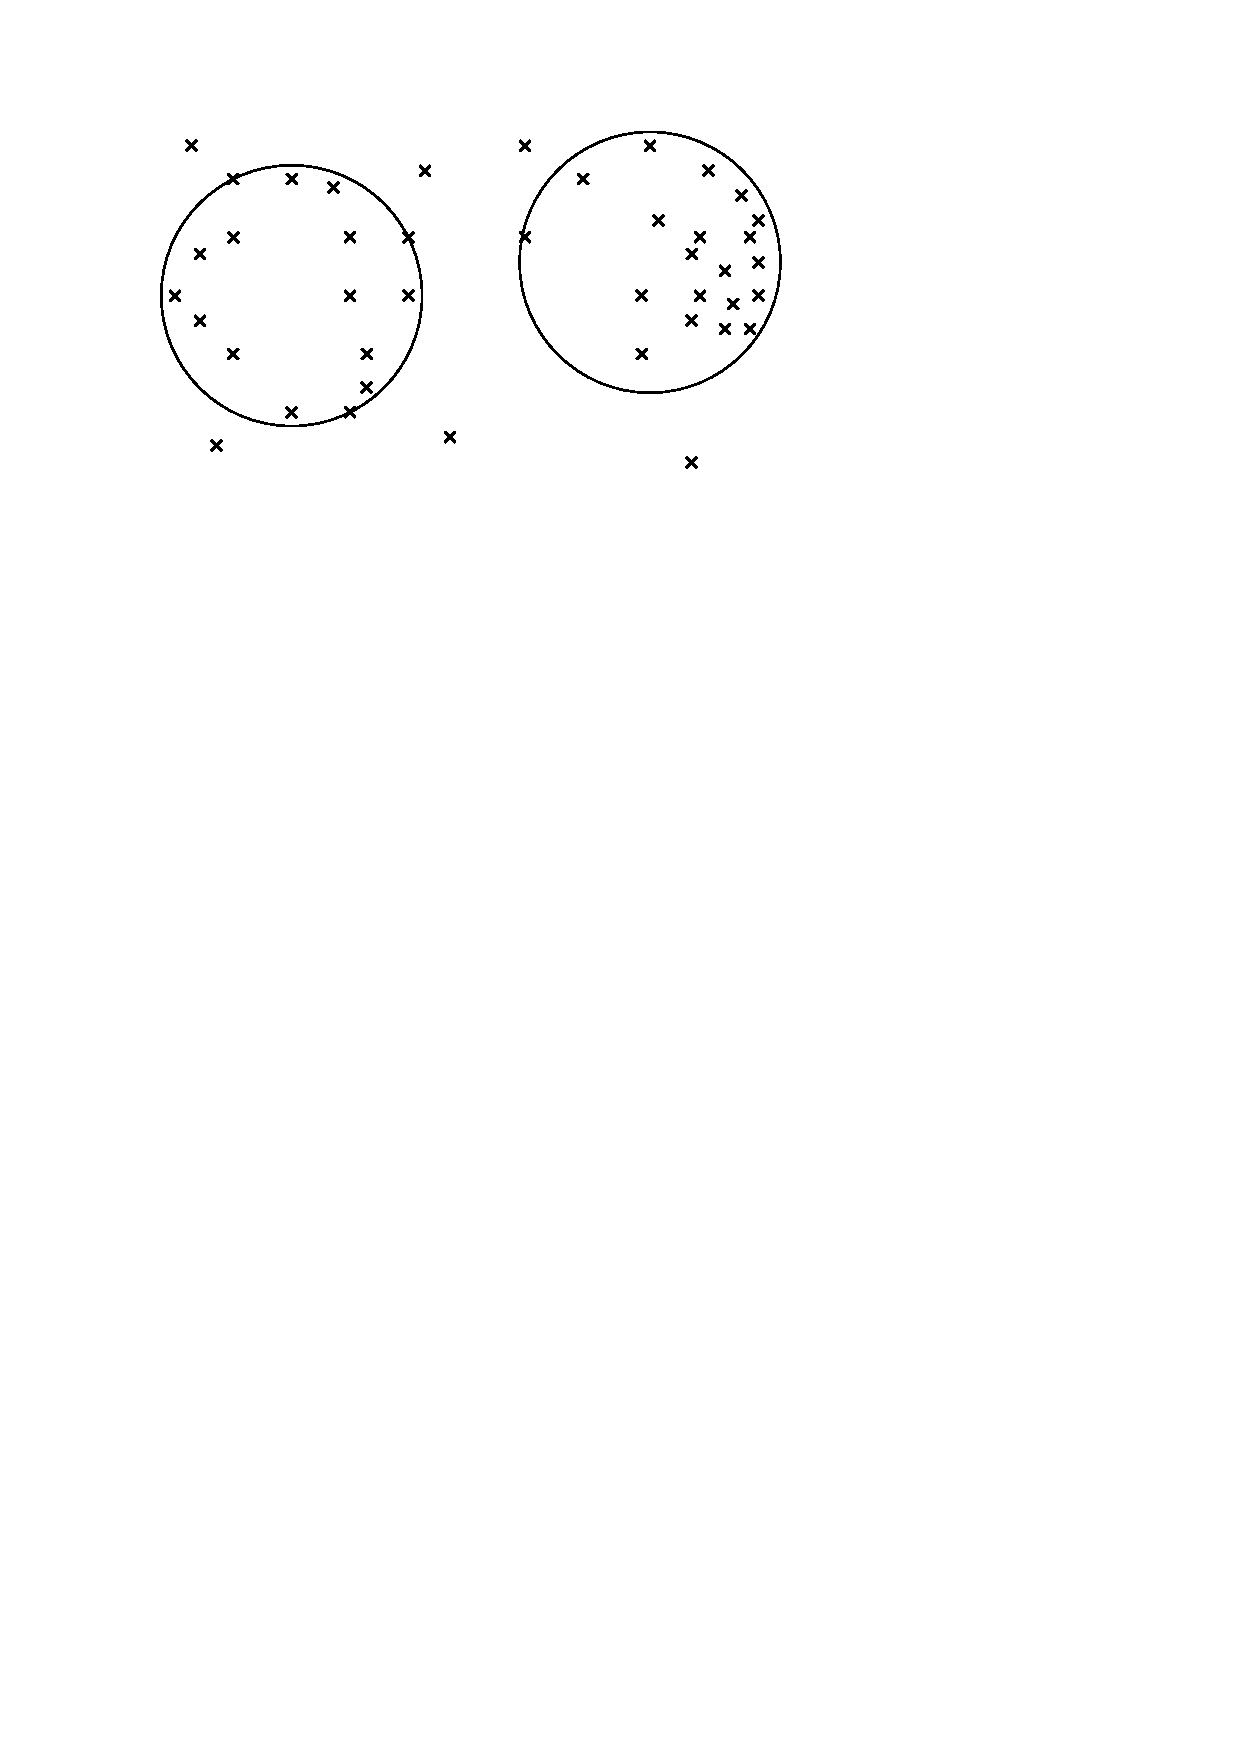
\includegraphics[width=13em]{figs/definition}
	\caption{An example of $2$-center with 6 outliers}
	\label{fig:definition}
\end{figure}

In the streaming model, McCutchen~\etal~\cite{mccutchen2008streaming} 
and Guha~\cite{guha2009tight} presented algorithms to maintain $(2+\eps)$-approximation 
to the $k$-center problem in %in any metric space using 
$\O(\frac{kd}{\eps} \log \frac{1}{\eps})$ space.
For $k=1$, %better algorithms are known. % in high dimensions.
%a $1.5$-approximation in high dimensions was presented by Zarrabi-Zadeh and Chan~\cite{zarrabi2006simple}.
a factor-$((1+\sqrt{3})/{2})$ approximation 
was presented by Agarwal and Sharathkumar~\cite{agarwal2010streaming} 
in high dimensions, using $O(d)$ space. 
The approximation factor was later improved 
%to $(1+\sqrt{3})/{2}$ by Agarwal and Sharathkumar~\cite{agarwal2010streaming} 
to $1.22$ by Chan and Pathak~\cite{chan2014streaming}.
%If the dimension is fixed, a $(1 + \eps)$-approximation
%can be maintained in $\O({k}/{\eps^{((d-1)/2)}})$ space 
%using the notion of core-sets~\cite{zarrabi2008core}., 
%Ahn~\etal~\cite{ahn2014computing} gave a $(2+\eps)$-approximation algorithm using $\O(\frac{d}{\eps})$ space and update time, which was improved for Euclidean spaces by 
For $k=2$, Kim and Ahn~\cite{kim2014improved} 
have recently obtained a $(1.8+\eps)$-approximation  
using $\O(\frac{d}{\eps})$ space and update time.

For $k$-center with $z$ outliers in the streaming model, 
McCutchen~\etal~\cite{mccutchen2008streaming} 
%(using the idea in Charikar~\etal~\cite{charikar2001algorithms} as subroutine) 
gave a $(4+\eps)$-approximation 
%(or $(3+\eps)$-approximation, if all center points can be enumerated) 
algorithm using $\O(\frac{zk}{\eps})$ space.
When dimension is fixed, a $(1 + \eps)$-approximation to 1-center with outliers
can be maintained in $\O({z}/{\eps^{((d-1)/2)}})$ space 
using the notion of robust $\eps$-kernels~\cite{agarwal2007space, zarrabi2011almost}.
For 1-center with outliers in high dimensions, 
Zarrabi-Zadeh and Mukhopadhyay~\cite{zarrabi2009streaming} 
gave a $(\sqrt{2}\alpha)$-approximation, 
where $\alpha$ is the approximation factor of the underlying algorithm for maintaining 1-center. 
Combined with the $1.22$-approximation algorithm of Chan and Pathak~\cite{chan2014streaming},
it yields an approximation factor of $(\sqrt{2} \times 1.22) < 1.73$ 
using $O(d^3z)$ space and $\poly(d,z)$ update time.
%In fixed dimensions, there is a streaming $\O(\frac{z}{\eps^{\O(d)}})$-space algorithm~\cite{agarwal2007space, zarrabi2011almost}.


\begin{table}[t]
\centering
\begin{tabular}{|c|c|c|}
\hline
\multirow{2}{*}{\begin{tabular}[c]{@{}c@{}} \ \  Problem \ \ \end{tabular}} & \multicolumn{2}{c|}{Approximation Factor} \\ \cline{2-3} 
 & Without Outliers & With Outliers \\ \hline \hline
1-Center & 1.22~\cite{chan2014streaming} & 1.73~\cite{zarrabi2009streaming} \\ \hline
2-Center & $1.8 + \eps$~\cite{kim2014improved} & \textbf{$1.8 + \eps$} [Here]  \\ \hline
$k$-Center & $2 + \eps$~\cite{guha2009tight,mccutchen2008streaming} & $4 + \eps$~\cite{mccutchen2008streaming}  \\ \hline
\end{tabular}
\caption {Summary of the streaming algorithms 
for $k$-center with and without outliers in high dimensions.}
\label{table:summary}
\end{table}

\paragraph{Our result}
In this paper, we study the 2-center problem with outliers in high dimensions.
We present a streaming algorithm for the problem that achieves
an approximation factor of $1.8 + \eps$, for any $\eps > 1$,
%using $O(d^3z/\eps)$ space.
using $\poly(d, z, {1 \over \eps})$ space and update time.
This improves the current streaming algorithm available for the problem
which has an approximation factor of $4+\eps$.
%Our work not only improves the best previous algorithm available for the case of 2-center,
%but is also counterintuitive in the sense that its 
The approximation factor of our algorithm matches
that of the best streaming algorithm for the 2-center problem without outliers.
This is somewhat surprising, considering that 
the best current approximation factors for streaming $k$-center with and without outliers 
differ by a factor of $\sqrt{2}$ for $k=1$,
and by a factor of 2  for general~$k$. %the 1-center problem.
See \Cref{table:summary} for a comparison.

To obtain our result, we have used a combination of several ideas
including parallelization construction, far/close ball separation,
and keeping a lower bound on the radius and distance of the optimal balls.
We have also utilized ideas used in~\cite{kim2014improved} 
for the 2-center problem with no outliers.
%However, our algorithm is much detailed and uses many new ingredients.
However, our problem is much harder here, % handling outliers makes the problem much harder,
as we not only need to find balls of minimum radius, 
but we also need to decide which subset of points to cluster.
This is in particular more challenging in the streaming model,
where we only have a single pass over the input, and we must decide on the fly
which point is an outlier, 
and which one can be safely ignored as a non-outlier point,
%using only a limited amount of storage.
to comply with the working space restriction enforced by the model.


\REM{
The rest of this paper is organized as follows.
In Section~\ref{sec:1-center}, we give a simple $2$-approximation algorithm for 
the 1-center problem with outliers that uses $\O(z^2 + zd)$ space.
In the next section, we show a $(1.8 + \eps)$-approximation
streaming algorithm for 2-center with $z$ outliers in high dimensions. 
}


% ---------------------------- Preliminaries -------------------------------

\section{Preliminaries}
\label{sec:pre}
Let $B(c,r)$ denote a ball of radius $r$ centered at $c$. 
We use $r(B)$ to denote the radius of a ball $B$. % and $c(B)$, respectively.
For two points $p$ and $q$, %by $pq$ the straight line segment between $p$ and $q$,
the distance between $p$ and $q$ is denoted by $\len{pq}$.
Given two balls $B(c,r)$ and $B'(c',r')$, 
we define 
$\delta(B, B') = \max \set{0, \len{cc'}-r-r'}$
to be the \emph{distance} between $B$ and $B'$.
Two balls $B_1$ and $B_2$ %with radius $r$ 
are said to be \emph{$\alpha$-separated}, 
%if $\delta(B_1, B_2) \geq \alpha r$.
if $\delta(B_1, B_2) \geq \alpha \cdot \max \set{r(B_1), r(B_2)}$.


Given an $n$-point set $P$ in $d$-dimensions,
a point $c \in \IR^d$ is called a \emph{centerpoint} of $P$,
if any halfspace containing $c$ contains at least $\ceil{{n}/({d + 1})}$ points of $P$. 
%In other words, any halfspace (or convex set) that avoids a centerpoint can contain at most $\floor{\frac{dn}{d + 1}}$ points of $P$. 
It is well-known that any finite set of points in $d$-dimensional space 
has a centerpoint~\cite{danzer1963helly}. 
The following observation is a corollary of this fact.
%~\cite{edelsbrunner1987algorithms}.

\begin{obs}
\label{obs:omitting-centerpoint}
	Given a set $P$ of $k(d+1)$ points in $d$-dimensional space, 
	the centerpoint of $P$ has the property that 
	any convex object not covering the centerpoint, 
	leaves at least $k$ points of $P$ uncovered.
\end{obs}

Given  a point set $P$,
the \emph{$k$-furthest point from} $p \in P$
is a point whose distance to $p$ is the $k$-th largest among all points in $P$.
%is the $k$-th point in $P$ when points are sorted
%in their decreasing distance from~$p$.
We assume the standard word-RAM model of computation. 
Each coordinate value takes a unit of space.
Thus, a $d$-dimensional point takes $\O(d)$ space,
and basic operations on the points take $\O(d)$ time.


%-------------------------- 1-center ---------------------------------

\section{A Simple Algorithm for 1-Center with Outliers}
\label{sec:1-center}

To warm up, we present a simple $2$-approximation streaming algorithm
for the 1-center problem with outliers.
It utilized a parallelization technique that 
will be used extensively in the rest of the paper.
The pseudocode is provided in \Cref{alg:1-center}.
The algorithm receives as input a stream of points, $P$,
and the number of outliers, $z$.
It also assumes that the first point $p_1$ of the stream is non-outlier.
We will show later how to remove this assumption.
The algorithm returns a ball $B$ covering all but at most $z$ points of $P$.
%

%\begin{algorithm}
%\caption{\sc 1-Center$(P, z)$} 
%\algsetup{indent=1.5em}
%\label{alg:1-center}
%\begin{algorithmic}[1]
%
%	%\STATE Let $p_i$ denote the elements of $P$, for $i \in \set{1, \dots, n}$.
%	\STATE let $p_1, \ldots, p_n$ be the points of $P$
%	\FOR{$i = 1, \dots, z+1$}
%		%\STATE move $p_i$ to the front of $P$ %is a non-outlier point in optimal solution.
%		\STATE $B_i \gets$ \Call{1-Center-Special}{$P, z,p_i$}
%	\ENDFOR
%	%\STATE $i^* \gets \argmin_{i=1}^{z+1} r_i$
%	\RETURN smallest ball among $\set{B_1, \ldots, B_{z+1}}$
%
%\end{algorithmic}
%\end{algorithm}

\begin{algorithm}
\caption{\sc 1-Center$(P, z)$} 
\algsetup{indent=1.5em}
\label{alg:1-center}
\begin{algorithmic}[1]
	%\STATE {$\triangleright$ $c$ is a non-outlier point in the optimal solution}
	\STATE $B \gets B(p_1, 0)$
	\STATE $Q \gets \emptyset$
	\FORALL {$p$ in $P$}
		\IF {$p \notin B$}
			\STATE insert $p$ into $Q$
			\IF {$|Q| = z + 1$}
				\STATE $q$ $\gets$ closest point to $c$ in $Q$
				\STATE remove $q$ from $Q$
				\STATE $B \gets B(c, \len{cq})$
			\ENDIF
		\ENDIF
	\ENDFOR
	\RETURN {B}
\end{algorithmic}
\end{algorithm}

%The function \textproc{1-Center-Special} in \Cref{alg:1-center-special}, 
%takes as input a point $c$ which is guaranteed to be a non-outlier point in the optimal solution. 
%To overcome the lack of knowledge about such a point, 
%function \textproc{1-Center} in \Cref{alg:1-center}
%tries each of the first $z+1$ points of the stream as a candidate for a non-outlier point and 
%generates a ball for each, using function \textproc{1-Center-Special}. 
%It returns the ball with the minimum radius. 
%Note that, in the streaming model, %due to space limitations inherent to streaming data model, 
%the body of the for loop in function \textproc{1-Center} runs in parallel.
%To run function \textproc{1-Center} in the data stream model,
%we run the body of the for loop in $z+1$ parallel streaming instances.

\begin{theorem} \label{thm:1-center}
	Algorithm~\ref{alg:1-center} computes a $2$-approximation to
	the 1-center problem with $z$ outliers,
	assuming that the first point of the stream is not outlier. 
\end{theorem}


\begin{proof}
Let $B^*(c^*, r^*)$ be the optimal solution,
and $c = p_1$ be a non-outlier point in the optimal solution.
Since $c$ is covered by $B^*$,
for all points $p \in B^*$, we have
$\len{cp} \le \len{cc^*} + \len{c^*p} \le 2r^*$.
Among the $z+1$ points furthest from $c$,
there is at least one point $q$ which is not outlier, % in the optimal solution,
and therefore, is contained in $B^*$
(see \Cref{fig:1center}). 
Thus, $\len{cq} \le 2r^*$,
and hence, the ball $B(c, \len{cq})$ returned by Algorithm~\ref{alg:1-center} 
is a 2-approximation. 
\end{proof}


\begin{figure}[t]
	\centering
	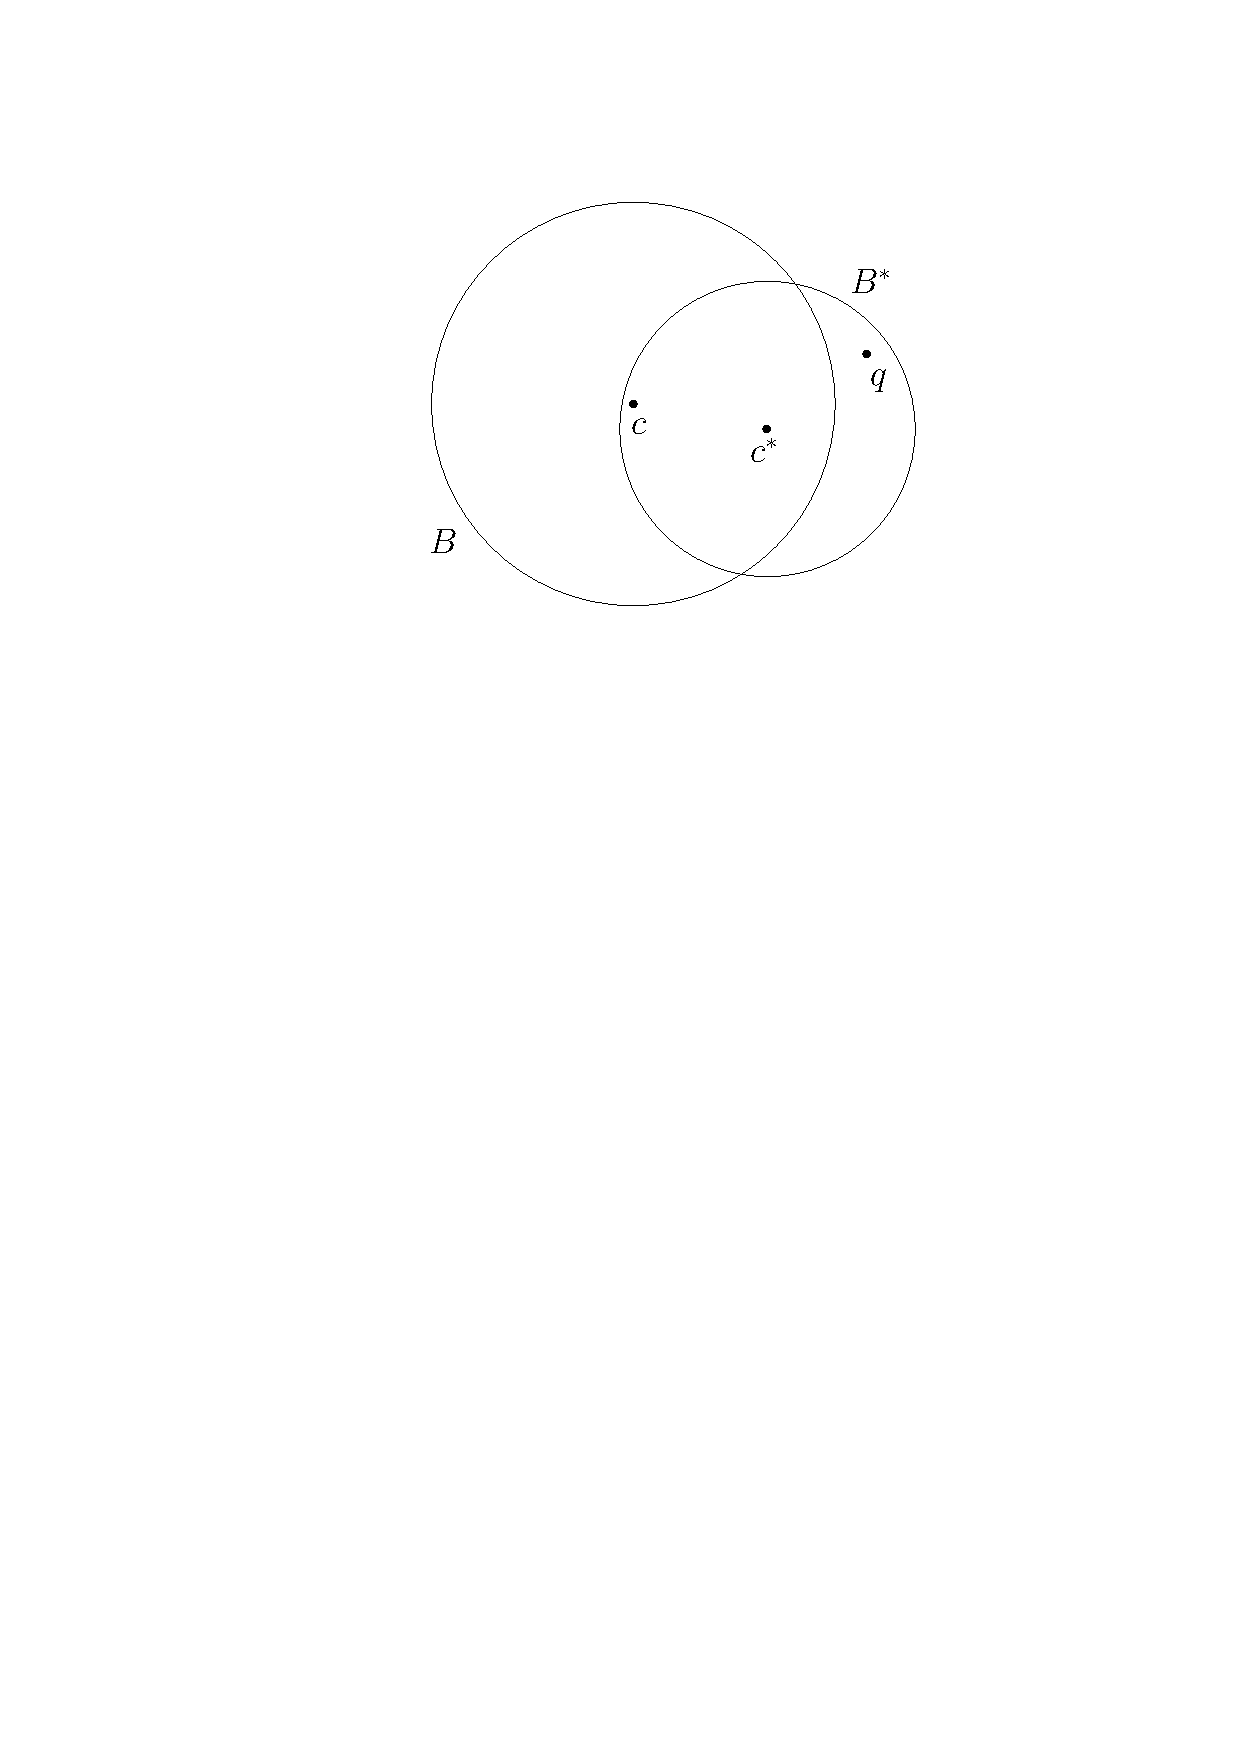
\includegraphics[width=10em]{figs/one-center}
	\caption{Proof of \Cref{thm:1-center}}
	\label{fig:1center}
\end{figure}


\noindent
Algorithm~\ref{alg:1-center} 
assumes that the first point of the stream is not outlier.
To remove this assumption,
we run $z+1$ instances of \Cref{alg:1-center} in parallel,
each of which is given as input one of the first $z + 1$ points of the stream,
followed by the rest of the points.
Clearly, there exists a point among the first $z+1$ points of $P$
which is not an outlier in the optimal solution.
Therefore, the smallest ball among the $z+1$ balls computed in parallel
is always within factor~2 of the optimal solution. % by \Cref{thm:1-center-special}.
Since the space complexity of Algorithm~\ref{alg:1-center} for one instance is $\O(zd)$, 
and its update time is $\O (zd \log z)$, % and the query time is $\O (z)$.
we get the following result.

\begin{theorem} \label{thm:1-center-stream}
	Given a stream of points in $d$ dimensions,
	we can maintain a 2-approximation to the 1-center with $z$ outliers
	in $\O(z^2d)$ space and $\O (z^2d\log z)$ update time.
\end{theorem}

%function \textproc{1-Center} in \Cref{alg:1-center}
%tries each of the first $z+1$ points of the stream as a candidate for a non-outlier point and 
%generates a ball for each, using function \textproc{1-Center-Special}. 
%It returns the ball with the minimum radius. 
%Note that, in the streaming model, %due to space limitations inherent to streaming data model, 
%the body of the for loop in function \textproc{1-Center} runs in parallel.
%To run function \textproc{1-Center} in the data stream model,
%we run the body of the for loop in $z+1$ parallel streaming instances.
%
%The space complexity of Algorithm~\ref{alg:1center} is $\O(z^2 + zd)$, the update time is $\O (z \log z + zd)$ and the query time is $\O (z)$.
%If a non-outlier point $p$ is known then the space, update time and query time complexities of Algorithm~\ref{alg:1center} can be reduced by a factor of $z$.



%-------------------------- 2-center ---------------------------------



\section{The 2-Center Problem with Outliers}
\label{sec:2-center}

In this section, we provide a $(1.8 + \eps)$-approximation algorithm
for the 2-center problem with outliers.
In all algorithms presented in this section,
we assume that the first point of the stream, $p_1$, is non-outlier. 
This assumption can be easily removed by considering $z + 1$ parallel instances of the algorithm, 
similar to what we did in \Cref{sec:1-center}.

Let $B_1^*$ and $B_2^*$ be the balls
in an optimal solution to the 2-center problem with $z$ outliers on a point set $P$.
We denote by $r^*$ the optimal radius,
and by $\delta^*$ the distance between $B_1^*$ and $B_2^*$.
To prove our main result, we distinguish between two cases.
In \Cref{subsec:bigger}, we address the case where $\delta^* > \alpha r^*$, 
for some constant $\alpha$ to be fixed later.
(It will turn out that $\alpha = 16$ is a proper choice.)
We then present in \Cref{subsec:smaller} 
our algorithm for the case of $\delta^* \leq \alpha r^*$.

%We inspect the case where $\delta^* \ge \alpha r^*$ in Subsection~\ref{subsec:bigger}.
%give a description of our algorithm for a given $r > 0$ for the case where $\delta^* < \alpha r^*$ and $1.2r^* \le r < (1.2 + 2\eps/3)r^*$, which returns a $(1.8 + \eps)$-approximate solution. We explain how to find such an $r$ and present a full description of our algorithm for the case where $\delta^* < \alpha r^*$ in Subsection~\ref{subsec:findr}. 




% -------------------------------- First Case -----------------------------------

\subsection{The Case $\delta^* > \alpha r^*$}
\label{subsec:bigger}

In this section, we present a $1.8$-approximation algorithm for the case 
where optimal balls are separated by a distance greater than $\alpha r^*$.
We start by two useful observations.
%The value of $\alpha$ will be fixed later in this section.  

\begin{obs}
\label{obs:c+4}
	Let $B_1$ and $B_2$ be two congruent balls of radius $r$,
	with distance $\delta > \alpha r$.
	%If $p$ and $q$ are two points in $B_1$ and $B_2$, respectively,
	For any two points $p \in B_1$ and $q \in B_2$,
	we have $1 \le \frac{\len{pq}}{\delta} <  \frac{\alpha + 4}{\alpha}$.
\end{obs}

\begin{proof}
The distance between $p$ and $q$ is at most $\delta + 4r$.
%(see \Cref{fig:c+4}).
Hence, $\frac{\len{pq}}{\delta} \leq 1 + {4r \over \delta} < 1 + \frac{4}{\alpha}$.
\end{proof}

\REM{
\begin{figure}[th]
	\centering
	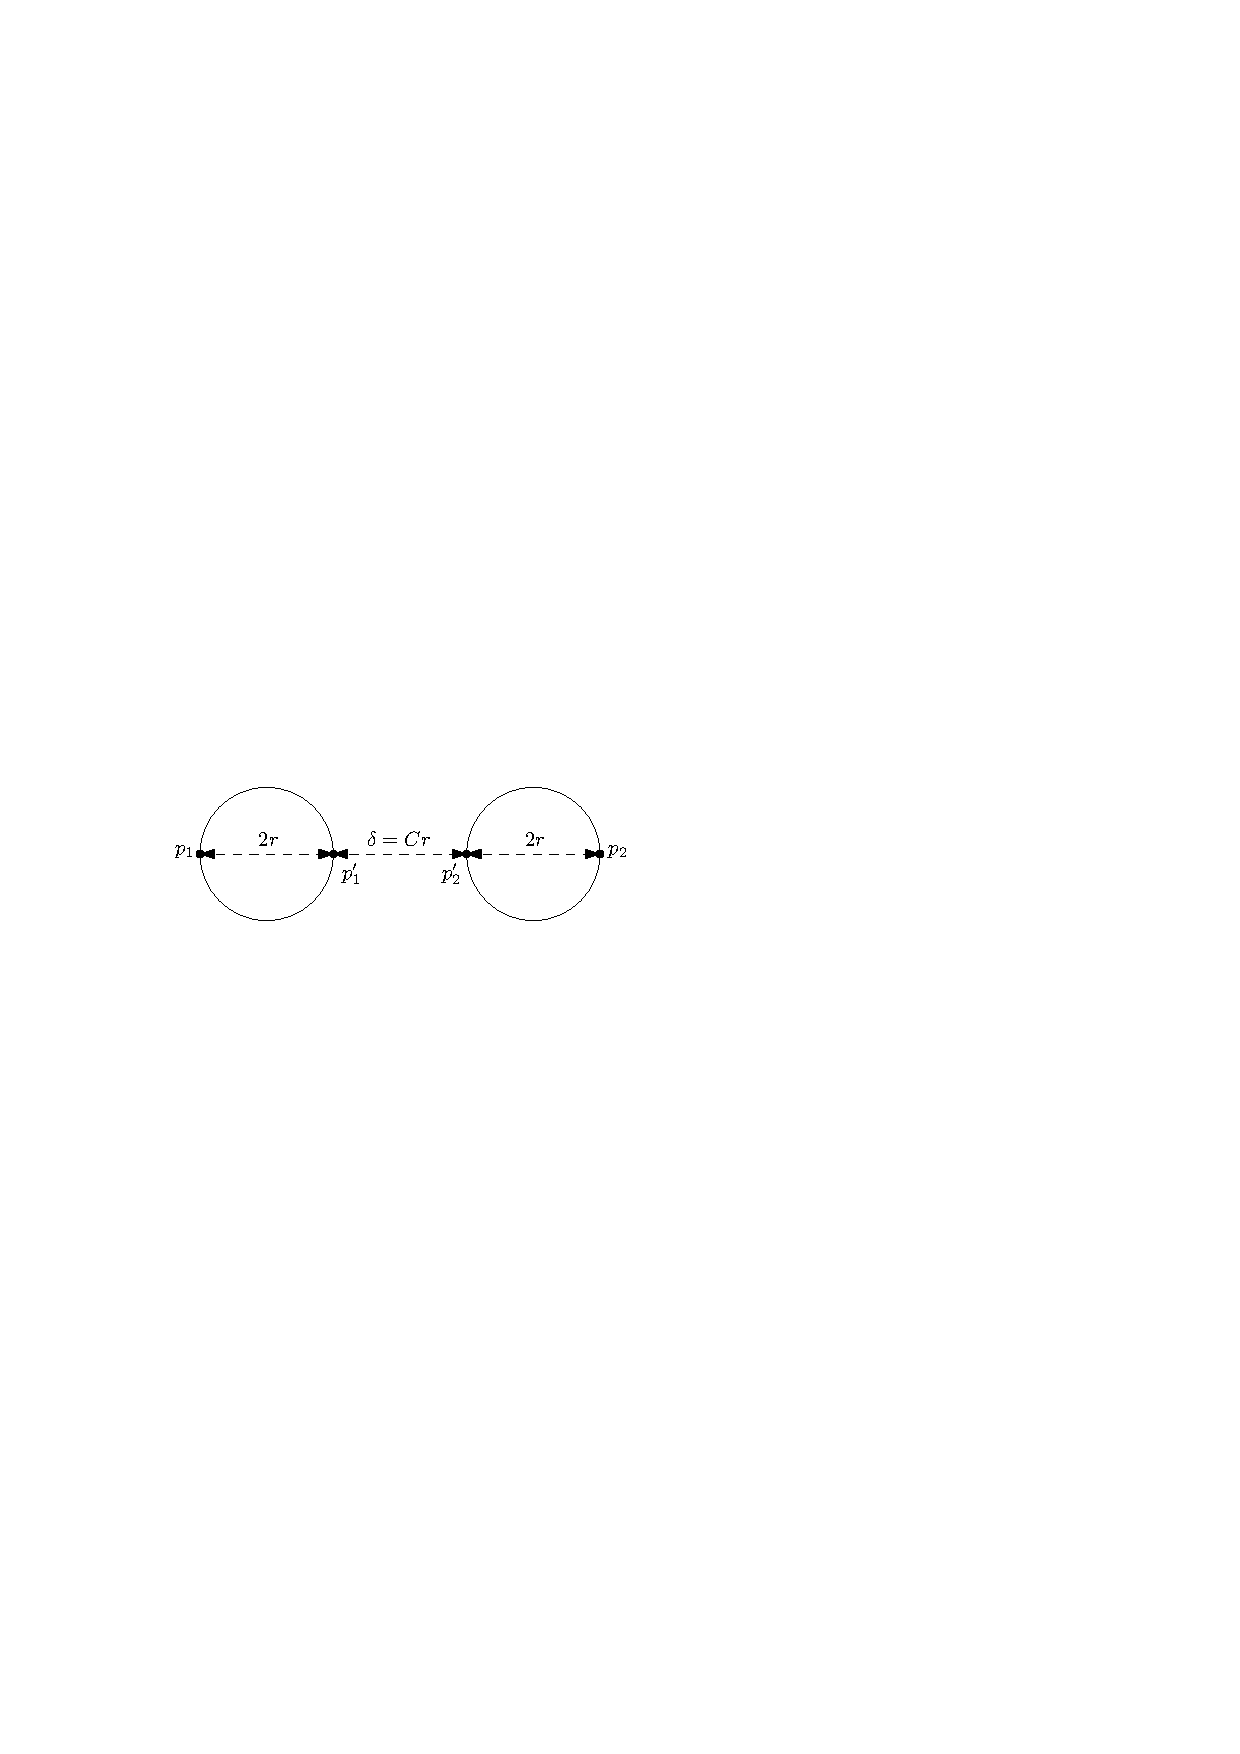
\includegraphics[width=20em]{figs/c_plus_4}
	\vspace{-1em}
	\caption{Illustrating Observation~\ref{obs:c+4}}
	\label{fig:c+4}
\end{figure}
}

\begin{obs}
\label{obs:intersection}
	Let $B_1$ and $B_2$ be two disjoint balls of distance $\delta$,
	and let $B$ be an arbitrary ball of radius less than $\frac{\delta}{2}$. 
	Then $B$ intersects at most one of $B_1$ and $B_2$.
\end{obs}

\noindent 
%Before presenting our algorithm,
We next prove some properties regarding 
the optimal balls, $B_1^*$ and $B_2^*$.

\begin{lemma}
\label{lem:c-sep}
	Let $B_1^*$ and $B_2^*$ be $\alpha$-separated, with $\alpha > 4$.
	If $p$ is a point in $B_1^*$,
	and $S$ is a $(z+1)$-subset of $P$ furthest from~$p$,
	then $S \cap B_2^*$ is non-empty.
\end{lemma}

\begin{proof}
Suppose by way of contradiction that $S \cap B_2^*$ is empty. 
Since $\card{S} = z + 1$, there is at least one point in $S$
which is not outlier, and hence, it is in $B_1^*$.
Let $q$ be the point in $S \cap B_1^*$ furthest from~$p$. 
Consider $B(p, \len{pq})$. It is clear that $B$ covers $P \setminus S$. 
Since $p, q \in B_1^*$, then $\len{pq}$ is at most $2r^*$. 
Thus, by Observation~\ref{obs:intersection}, $B_2^* \cap B = \emptyset$. 
Therefore, $B_2^* \cap P = \emptyset$, and hence,
 $B_2^*$ is empty, which contradicts the optimality of the solution.
\end{proof}

\begin{lemma}
\label{lem:(z+1)-furthest}
	Let $p$ be a point in $B_1^{*}$,
	and $q$ be the $(z+1)$-furthest point from $p$. 
	Then, $\delta^* > \frac{\alpha}{\alpha+4}\len{pq}$.
\end{lemma}

\begin{proof}
By Lemma~\ref{lem:c-sep}, there exists a point $q' \in B_2^*$ 
such that $\len{pq'} \ge \len{pq}$. 
Thus, by Observation~\ref{obs:c+4}, 
%$\frac{\alpha}{\alpha+4} \len{pp_2} \le \delta^*$. 
${\len{pq} \over \delta^*} \le {\len{pq'} \over \delta^*} < \frac{\alpha+4}{\alpha}$.
\end{proof}

\begin{lemma}
\label{lem:2r}
	If $p \in B_1^*(c_1, r^*)$ and $q \in B_2^*(c_2, r^*)$,
	then $B_1^* \subset B(p, 2r^*)$ and $B_2^* \subset B(q, 2r^*)$,
	and hence, at most $z$ points of $P$ lie outside $B(p, 2r^*) \cup B(q, 2r^*)$.
\end{lemma}

\begin{proof}
	For an arbitrary point $p' \in B_1^*$, $\len{pp'} \leq \len{pc_1} + \len{p'c_1} \leq 2r^*$,
	and as a result, $B_1^* \subset B(p, 2r^*)$.
	Similarly, we have $B_2^* \subset B(q, 2r^*)$. 
	Considering that at most $z$ points of $P$ are outlier, the proof is complete.
\end{proof}

\begin{lemma}
\label{lem:center-point}
	Let $S$ be a subset of $P$ of size at least $\dz$,
	enclosed by a ball $B$ of radius less than $\delta^* / 2$.
	Then the centerpoint $c_p$ of $S$ lies inside either $B_1^{*}$ or $B_2^{*}$.
\end{lemma}

\begin{proof}
	Not all points in $S$ can be outlier, because $\dz > z$.
	Thus, by Observation~\ref{obs:intersection},
	$B$ intersects exactly one of $B_1^*$ and $B_2^*$.
	Assume, w.l.o.g., that $B$ intersect $B_1^*$. 
	Now, by Observation \ref{obs:omitting-centerpoint}, 
	if $c_p$ is not in $B_1^*$, 
	then $z+1$ points of $S$ remain uncovered by $B_1^*$,
	contradicting the fact that there at most $z$ outliers.	
\end{proof}

\paragraph{The Algorithm}
We now describe our algorithm for handling the case  $\delta^* > \alpha r^*$.
At any time, our algorithm maintains a partition of $P$ into three disjoint subsets
$B_1$, $B_2$, and Buffer.
The first point $p_1$ is assumed, w.l.o.g, to be in $B_1^*$. 
(We have already assumed that $p_1$ is not outlier.)
The algorithm tries to partition points in such a way that 
at the end,
$B_1$ contains the whole $B_1^*$, and $B_2$ contains the whole $B_2^*$,
with possibly some outliers being contained in $B_1$ and $B_2$.
%Buffer has always size at most $z$.
The algorithm sets $c_1 = p_1$ as the fixed center of $B_1$,
and picks $c_2$ among the points processed so far as a candidate 
for being the center of $B_2$.
Moreover, the algorithm maintains two values $\delta$ and $r$,
where at any time, $\delta$ is a lower bound of $\delta^*$, 
and $r$ is an upper bound of $2r^*$ (under a specific condition). %(if $c_p \in B_2^*$).

Our algorithm is presented in \Cref{alg:case-1}.
For each input point $p \in P$, the algorithm first tries 
to add $p$ to either $B_1$ or $B_2$,
using functions \textproc{AddToB$_1$} and \textproc{AddToB$_2$}, respectively.
%presented in Algorithms~\ref{alg:addB1} and~\ref{alg:addB2}.
If none of them fits, the point is added to Buffer.
The function \textproc{AddToB$_1$} adds a point $p$ to $B_1$
only if it is within distance $\delta$ of the center $c_1$.
Similarly, \textproc{AddToB$_2$} adds a point $p$ to $B_2$
only if it is within $\rc$-radius of $c_2$. 
The two functions also update the values of $\delta$ and $\rc$ whenever necessary,
to maintain the invariants to be defined in Lemma~\ref{lem:invariants}.


\begin{algorithm}[t]
\caption{\sc 2-CenterCase1$(P)$} 
\algsetup{indent=1.5em}
\label{alg:case-1}
\begin{algorithmic}[1]
\STATE $c_1 \gets p_1$, $\rc  \gets 0$, $\delta \gets 0$
\FORALL{$p \in P$}
	\IF {\NOT (\Call{AddToB$_1$}{$p$} \OR \Call{AddToB$_2$}{$p$})}
		\STATE add $p$ to Buffer
		\WHILE{$\card{\mbox{Buffer}} > z$} \label{step:buffer-overflow}
			\IF{$\card{B_2} \ge \dz$}
				\STATE $B_1 \gets B_1 \cup B_2$, $B_2 \gets \emptyset$
			\ELSIF{$c_2$ is set}
				\STATE $B_1 \gets B_1 \cup \set{c_2}$ %, $B_u \gets B_u \cup \set{c_2}$
				%\STATE remove $c_2$ from $B_2$
			\ENDIF
			\STATE $T \gets \mbox{Buffer} \cup B_2 \setminus \set{c_2}$
			\STATE $B_2 \gets \emptyset$ 
%			\IF{first iteration of while}
%				\FOR{$p \in T$}
%					\IF{\Call{AddToB$_1$}{$p$}}
%						\STATE remove $p$ from $T$
%					\ENDIF
%				\ENDFOR
%			\ENDIF
			\STATE $c_2 \gets$ (z+1)-furthest point from $c_1$ in $T$ 
			\STATE $\rc  \gets \radius{c_2}$
			\FOR{$p \in T$}
				\STATE \Call{AddToB$_2$}{$p$}
			\ENDFOR				
			\STATE $\mbox{Buffer} \gets T \setminus B_2$
		\ENDWHILE
	\ENDIF
\ENDFOR
\end{algorithmic}
\end{algorithm}


\begin{algorithm}[ht]
\caption{\sc AddToB$_1(p)$} 
\algsetup{indent=1.5em}
\label{alg:addB1}
\begin{algorithmic}[1]

	%\STATE $q \gets c_1$
	\IF {at least $z + 1$ points have been processed}
		\STATE $q \gets$  $(z+1)$-furthest point from $c_1$
	\ELSE
		\STATE $q \gets c_1$
	\ENDIF
	\STATE $\delta \gets \frac{\alpha}{\alpha+4} \len{c_1q}$
	\IF {$p \in B(c_1, \delta)$}
		\STATE $B_1 = B_1 \cup \set{p}$ %, B_u = B_u \cup \set{p}$
		\RETURN{true}
	\ENDIF
	\RETURN{false}

\end{algorithmic}
\end{algorithm}

\begin{algorithm}[ht]
\caption{\sc AddToB$_2(p)$} 
\algsetup{indent=1.5em}
\label{alg:addB2}
\begin{algorithmic}[1]
%\FUNCTION{AddToB$_2$}{p}
	\IF{$c_2$ is set \AND $p \in B(c_2, \rc )$}
		\STATE $B_2 \gets B_2 \cup \set{p}$ %, B_u \gets B_u \cup \set{p}$
		\IF{$|B_2| = \dz$}
			%\STATE $\cp  \gets$  centerpoint of $B_2$
			\STATE $\rc  \gets  (2 + \frac{2}{\alpha}) \times \rc$
			\FOR{$p$ in Buffer}
				\IF{$p \in B(c_2, \rc )$}
					\STATE $B_2 \gets B_2 \cup \set{p}$ %, B_u \gets B_u \cup \set{p}$
					\STATE remove $p$ from Buffer
				\ENDIF
			\ENDFOR
		\ENDIF
		\RETURN{true}
	\ENDIF
	\RETURN{false}
%\ENDFUNCTION
\end{algorithmic}
\end{algorithm}

Whenever the buffer overflows (in line~\ref{step:buffer-overflow} of \Cref{alg:case-1}),
%the assumption about $\cp \in B_2^*$ is contradicted.
%At some point during the execution of Algorithm~\ref{alg:case-1}, the assumption about $\cp \in B_2^*$ might be contradicted when the buffer overflows. We can then conclude that
% $\cp \notin B_2^*$.
the algorithm takes one of the following actions
depending on the size of $B_2$. 
If $|B_2| \ge \dz$, then the points of $B_2$ are moved to $B_1$, and $B_2$ is reset.
Otherwise, the old $c_2$ (if already set) is moved to $B_1$,
and another point from $T = B_2 \cup \Buffer \setminus \set{c_2}$ is picked as $c_2$.
The while loop iterates at most $O(dz)$ times,
because after the first iteration, we are sure 
that $T$ has at most $\dz + z$ points, from which 
one point (i.e., $c_2$) is removed at each subsequent iteration.


%\paragraph{Analysis}
For the sake of analysis, we maintain a ``central point'', 
denoted by $\cp$, %not necessarily in $P$,
%which we call a \emph{central point}.
which is defined as follows:
if $\card{B_2} < \dz$, then $\cp = c_2$, otherwise,
$\cp$ is the centerpoint of the first $\dz$ points currently in~$B_2$.

\begin{lemma}
\label{lem:invariants}
	The following invariants are maintained during the execution of the algorithm:

\begin{enumerate}
\item [(a)] $\delta < \delta^*$ %$\delta$ is a lower bound of $\delta^*$
\item [(b)] if $c_2$ is set, then
\begin{enumerate}
	\item[1.] $r \leq \delta/2$
	\item[2.] $B(c_p, \radius{c_p}) \subset B_2(c_2, r)$
\end{enumerate}
\item [(c)] $B_1 \cap B_2^* = \emptyset$
\item [(d)]  if $\cp \in B_2^*$, then 
	\begin{enumerate}
		\item [1.] $2r^* \le r$
		\item [2.] $B_2 \cap B_1^* = \emptyset$
		\item [3.] all points in $\Buffer$ are outliers
	\end{enumerate}

\end{enumerate}
\end{lemma}

\begin{proof} 
%The proof consists of four parts and each part use previous parts:
Invariant (a): 
At the beginning, $\delta = 0$, which clearly satisfies the invariant.
After $z+1$ points of the stream is processed, 
function \textproc{AddToB$_1$} starts updating $\delta$
to $\frac{\alpha}{\alpha+4}\len{c_1q}$,
where $q$ is the $(z+1)$-furthest point from $c_1$ in the current stream.
Now, since $c_1 \in B_1^*$, Lemma~\ref{lem:(z+1)-furthest}
implies that $\delta < \delta^*$.
%Note that if less than $z+1$ points have been processed so far,
%then $\delta = 0$, and hence, the invariant holds.

Invariant (b1): 
When an appropriate candidate for $c_2$ is found, 
$c_2$ is set to that candidate by the main algorithm (Algorithm~\ref{alg:case-1}),
and $\rc$ is set to $\frac{2}{\alpha}\len{c_1c_2}$.
After that, points are added to $B_2$ by function \textproc{AddToB$_2$}
only if they are within $\rc$-radius of $c_2$. 

If $c_2$ is set, then it is the $(z+1)$-furthest point from $c_1$ in a set $T \subset P$.
Let q be the $(z+1)$-furthest point from $c_1$ in the stream at that state, then $\len{c_1c_2} \leq \len{c_1q}$ and since (for $16 \leq \alpha$) $\radius{c_2} \leq \frac{1}{6}\frac{\alpha \len{c_1 q}}{(\alpha + 4)} \leq \delta / 6$, then 
$$r \leq (2 + \frac{2}{\alpha})\radius{c_2} \leq 3 \radius{c_2}  \leq \delta /2.$$

In part 2, if $|B_2| < \dz$ then $c_p = c_2$ and $r = \radius{c_2}$, so $B_2 = B(c_p, \radius{c_p})$. 
When the size of $B_2$ reaches $\dz$, the central point $\cp$ moves to the centerpoint of $B_2$ and $\rc$ increases by a factor of $(2 + \frac{2}{\alpha})$. 
Because the centerpoint of $B_2$ locate in $B_2$, then $c_p \in B(c_2, \radius{c_2})$.
So if $|B_2| \ge \dz$ then $\len{c_2 c_p} \leq \radius{c_2}$ and as a result
$$\radius{c_p} \leq \frac{2 (\len{c_1 c_2} + \len{c_2 c_p})}{\alpha} \leq \radius{c_2}(1 + \frac{2}{\alpha})$$ 
So $B(c_p, \radius{c_p}) \subset B_2(c_2, \radius{c_2}(2 + \frac{2}{\alpha}))$.

Invariant (c): A point $p$ can be added to $B_1$ in two parts of the \Cref{alg:case-1}. 
First case is in function \textproc{AddToB$_1$}, the point will be added to $B_1$ only if it is within distance $\delta$ of the center $c_1$,  when $\len{pc_1} \leq \delta$, which due to invariant (a), guaranties $\len{pc_1} < \delta^*$, so $p \not \in B_2^*$.

Second case is in \Cref{alg:case-1}, whenever the buffer overflows and $B_2$ is non-empty the algorithm takes one of the following actions depending on the size of $B_2$.
If $|B_2| < \dz $, then $c_2 = c_p$. \Cref{alg:case-1} add $c_2$ to $B_1$.
By contradiction assume that $c_p \in B_2^*$, then due to invariant (b) part 1 and invariant (d) part 1, $2r^* \leq r \leq \delta/2 < \delta^*/2$. So by Lemma \ref{lem:2r}, there should be at most $z$ points outside $B_1 \cup B_2$ which contradicts overflow of the buffer. 

If $|B_2| \geq \dz$, then $c_p$ is the centerpoint of the first $\dz$ points currently in $B_2$. 
In this case, we add all points of $B_2$ to $B_1$. Due to invariant (b), $r \leq \delta/2 < \delta^*/2$. 
So By Lemma \ref{lem:center-point}, $c_p \in B_1^*$ or $c_p \in B_2^*$. By contradiction assume that $c_p \in B_2^*$. In this case, due to invariant (d) part 1 and invariant (b) part 2, $B_2$ covers $B(c_p, \radius{c_p})$ and $2r^* \leq r$. similar to previous part, it contradicts overflow of the buffer. 

Invariant (d): 
Due to  Observation \ref{obs:c+4}, if $c_1 \in B_1^*$ and $c_p \in B_2^*$ then $1 \leq \frac{\len{c_1 c_p}}{\delta^*} \leq \frac{\len{c_1 c_p}}{\alpha r^*}$ and as a result $2r^* \leq \radius{c_p}$. If $|B_2| < \dz$ then $c_p = c_2$ and By \Cref{alg:case-1}, $r = \radius{c_2}$, so $2r^* \leq r$.

If $|B_2| \ge \dz$ then similar to invariant (b): $$2r^* \leq \radius{c_p} \leq (1 + \frac{2}{\alpha})\radius{c_2} \leq (2 + \frac{2}{\alpha})\radius{c_2} = r$$

In part 2, due to previous part, if $c_p \in B_2^*$ then $2r^* \leq r \leq \delta /2$ and $c_p \in B_2$. Due to invariant (a) and Observation \ref{obs:intersection}, $B_2$ intersect only with $B_2^*$ and so $B_2 \cap B_1^* = \emptyset$.

In part 3, due to invariant (c) and invariant (d) part 1, $2r^* \leq r \leq \delta/2 < \delta^* /2$. So by Lemma \ref{lem:2r}, all points outside $B_1 \cup B_2$ are outliers.

\end{proof}

%\paragraph{Streaming Model}
To implement our algorithm in the streaming model,
we maintain the sets $B_1$ and $B_2$ 
in a data structure that supports adding points,
and gives a $\beta$-approximation to 1-center with $k$ outliers, for $k=0,\dots,z$.
Moreover, we maintain a set $B_u = B_1 \cup B_2$ in a similar data structure.
Note that these data structures do not need to maintain all the points. 
They only need to have a buffer of size $\dz$ that keeps the most recently added points.

\REM{
Suppose that our data structure for maintaining $B_1$, $B_2$ and $B_u$ uses $S(n,z,d)$ space, $T(n,z,d)$ update and $Q(n,z,d)$ query time. Note that by $Q_{o}(zd,z,d)$ we mean the query time for the offline 1-center problem with $z$ outlier in $d$ dimensions. The best known algorithm for 1-center without outliers is $1.22$-approximation by~\cite{chan2014streaming, agarwal2010streaming}. The buffering framework introduced in~\cite{zarrabi2009streaming} with $\O(dz^3 + (\frac{d}{\eps^3})\log(\frac{1}{\eps}))$ space complexity, can be used with this algorithm as subroutine to achieve a $(1.22\sqrt{2})$-approximation ($1.22\sqrt{2} < 1.8$) for 1-center problem with outliers.

\begin{theorem}
\label{thm:2nd-cmplx}
Space complexity of Algorithm~\ref{alg:case-1} is $\O(dz+S(n,z,d))$. It takes $\O^*(dzT(n,z,d))$ time for update. Query time in Algorithm~\ref{alg:query} is $\O(zQ(n,z,d) + dz(dz+zQ_o(zd,z,d)))$ and it returns two centers that guarantee a $(1.8 + \eps)$-approximation for 2-center problem with outliers.
\end{theorem}

\begin{proof}
The space complexity for this algorithm is derived from the space used by $B_1$, $B_2$, $B_u$ and the Buffer which is obviously $\O(dz+S(n,z,d))$. The while loop runs at most once for each point, so amortized time is $\O(zdT(n,z,d))$. The candidates in the Algorithm~\ref{alg:query} are at most $zd$ points  so the query time will easily follows.
\end{proof}
}

\begin{theorem}
\label{thm:far-cmplx}
	If $\delta^* > \alpha r^*$, a $1.8$-approximation to the 2-center problem with $z$ outliers 
	can be maintained in $O(d^3z^2)$ space and $\poly(d,z)$ update time.
\end{theorem}

\begin{proof}
Our data structures for maintaining $B_1$, $B_2$, and $B_u$
employ the streaming algorithm of~\cite{zarrabi2009streaming,chan2014streaming}
%To maintain an approximation to 1-center with $z$ outliers,
%we use the streaming algorithm of~\cite{zarrabi2009streaming}
%which combined with the %current best streaming algorithm for 1-center~\cite{chan2014streaming},
%result of~\cite{chan2014streaming},
which has an approximation factor of $1.22 \times \sqrt{2} <1.8$.
The algorithm of~\cite{zarrabi2009streaming}
uses $O(d^3z)$ space and $\poly(d,z)$ update time,
which implies the same bounds for \Cref{alg:case-1}.
Since we need to run $z + 1$ instances of \Cref{alg:case-1} in parallel, 
the space and update time is multiplied by a factor of $z$.
\end{proof}


% -------------------------------- Second Case -----------------------------------

\subsection{The Case $\delta^* \leq \alpha r^*$}
\label{subsec:smaller}

%Our algorithm for solving the problem in this case is based on two main ingredients.
Our idea in this section is to carefully adopt
the algorithm of Kim and Ahn~\cite{kim2014improved},
originally designed for maintaining an approximate 2-center.
To avoid duplication, we just sketch the main steps of their algorithm,
%without entering the details, 
and explain our modifications to it. 
Kim and Ahn's algorithm, which we refer to as the KA algorithm,
has 9 different states, shown in~\Cref{fig:dag}.
Depending on the points arrived so far, the algorithm is in one of the states.
%In each step one or many of the states can be valid and their algorithm considers all of them in parallel. 
In each state, the algorithm keeps at most two balls, as a candidate solution. 
A transition between the states occurs whenever a point not covered by any of the two balls arrive. 

The algorithm starts at node 1, and proceed through the transition graph as points arrive.
In some states, there is more than one state to follow,
and the algorithm has no prior information which one is the correct choice.
However, there are only three different paths to follow in the transition graph. 
%which is a DAG,
%consisting of only three different transition paths.  
%(paths from node 1 to node E) 
Hence, we can easily run three instances of the algorithm in parallel,
each of which follows one of the paths deterministically, 
to make sure that at any time, at least one of the instances is in a correct state.

\begin{figure}
\centering
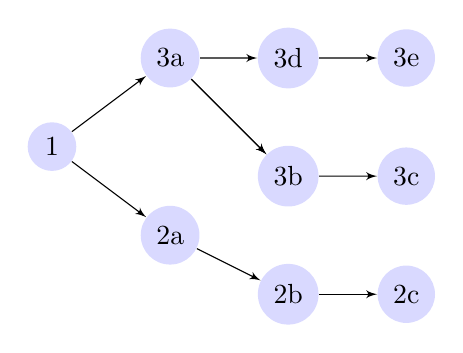
\begin{tikzpicture}
  [scale=.75,auto=left,every node/.style={circle,fill=blue!15}]
 \tikzset{edge/.style = {->,> = latex'}}
  \node (1) at (1,2.5) {1};
  \node (2a) at (3,1)  {2a};
  \node (3a) at (3,4)  {3a};
  \node (2b) at (5,0)  {2b};
  \node (3b) at (5,2)  {3b};
  \node (3d) at (5,4)  {3d};
  \node (2c) at (7,0)  {2c};
  \node (3c) at (7,2)  {3c};
  \node (3e) at (7,4)  {3e};
  %\node (E) at (9, 2) {E};

  \foreach \from/\to in {1/2a,1/3a,2a/2b,2b/2c,3a/3b,3a/3b,3a/3d,3b/3c,3d/3e} %,2c/E,3c/E,3e/E
    \draw[edge] (\from) to (\to);

\end{tikzpicture}
\caption{State diagram for the KA algorithm.
Labels are taken from \cite{kim2014improved}.}
\label{fig:dag}
\end{figure}

\newcommand{\state}{\text{state}}
\newcommand{\level}{{j}}
\newcommand{\counter}{\text{counter}}
\newcommand{\Insert}{\textsc{insert}}
\newcommand{\CA}{\text{KA}}

\begin{algorithm}[t]
\caption{\sc 2-CenterCase2$(P, z, r)$} 
\algsetup{indent=1.5em}
\label{alg:smallc}
\begin{algorithmic}[1]
	\STATE solutions $\gets \set{}$
	\FORALL {$(n_1, n_2, n_3, n_4)$ such that $\sum n_i=z$}
		%\FORALL {path $\pi$ in the transition graph}
		\FORALL {$\pi \in \set{1, 2, 3}$}
			\STATE $\counter_i \gets 0$, for $i = 1, \ldots, 4$ % $1 \le i \le 4$
			\STATE $B_1 \gets B(p_1, r)$, $B_2 \gets \emptyset$
			\STATE $\level \gets 1$ \COMMENT{$\level$ represents current level}
			\FORALL {$p \in P$}
				\IF {$p \not\in B_1 \cup B_2$}
					\STATE $\counter_\level \gets \counter_\level + 1$
					\IF {$\counter_\level > n_\level$}
						\STATE $\level \gets \level+1$
						\STATE $(B_1, B_2) \gets \CA.\Insert(p, \pi)$
					\ENDIF
				\ENDIF
			\ENDFOR
			\IF {$\level \le 4$}
				\STATE add $\max \set{r(B_1), r(B_2)}$ to solutions
				%\STATE add $(B_1, B_2)$ to solutions
			\ENDIF
		\ENDFOR
	\ENDFOR
	\RETURN $\min\set{\text{solutions}}$
\end{algorithmic}
\end{algorithm}

Our modification is on the transition part.
Points that are covered by the current solution can be safely ignored, 
as they do not cause any change in the current solution, and hence, they cause no transition.
Only those points that lie outside the current solution are candidates for being outliers.
Since the number of outliers in each state is unknown,
we try all possible choices. 
The observation here is that the transition graph is a DAG of depth four.
If $n_i$ ($1 \le i \le 4$) represents the number of outliers in depth $i$, 
then it suffices to consider all tuples $(n_1,\dots, n_4)$ such that $\sum_{i=1}^{4} n_i=z$,
It is easy to verify that there are $O(z^3)$ such tuples.

The pseudocode of our algorithm is presented in \Cref{alg:smallc}.
For each possible choices of $n_1$ to $n_4$, 
and each of the three paths in the transition graph, numbered from 1 to 3,
the algorithm keeps a candidate solution $(B_1, B_2)$ to the 2-center of non-outlier points,
a parameter $\level$ representing the current level in the transition graph,
and four counters to keep track of number of outliers seen so far at each level.

The algorithm starts with $B_1 = B(p_1, r)$ and $B_2 = \emptyset$,
which corresponds to Case 1 of the KA algorithm.
For each new point $p$, we first check if it is contained in the current solution.
If so, then we are done.
Otherwise, if the number of outliers seen in the current level has not yet reached $n_\level$, 
we consider $p$ as an outlier and proceed.
%If our quota for consuming outliers in this level is finished, 
Otherwise, we go to the next level, and update the current candidate solution, 
$(B_1, B_2)$, using the KA algorithm.
We give the transition path $\pi$ along with the point $p$ to the KA algorithm
to help it deterministically decide which state to choose as the next one.

After all points in $P$ are processed, if we are in one of the four states in the current path,
then the obtained solution is added to the feasible solutions.
Otherwise, the solution is not feasible, and is abandoned as in the KA algorithm.
Finally, we return the best solution among all computed feasible solutions. 
Kim and Ahn~\cite{kim2014improved} proved that in all feasible solutions
computed this way,
the larger ball among $B_1$ and $B_2$ has radius at most $3/2r$,
provided $\delta^* \le \alpha r^*$.
Assuming that we have a good estimate $r$ satisfying
$1.2r^* \le r < (1.2 + 2\eps/3)r^*$,
we get the following result.

\begin{theorem} \label{thm:close}
	For $1.2r^* \le r < (1.2 + {2 \over 3}\eps)r^*$ and $\delta^* \le \alpha r^*$,
	\Cref{alg:smallc} computes a $(1.8+\eps)$-approximation to 
	the 2-center with $z$ outliers 
	in $\O (dz^3)$ space and $\O (dz^3)$ update time.
\end{theorem}

\REM{
\begin{proof}
Since our algorithm considers all possible input cases of streaming points, there is at least one feasible solution. Since every feasible solution has its larger radius at most $3r/2$, the final solution has larger radius at most $3r/2 \le (1.8 + \eps)r^*$.
For space complexity, our algorithm maintains at most two balls in each case, and therefore it uses $\O(dz^3)$ space. Whenever the next point is inserted, the algorithm updates the solution for each subcase in $\O (d)$ time. Therefore, the algorithm spends $\O (dz^3)$ update time for each point of $P$. Answering a query consists of choosing the minimum radius among all the candidate solutions, which amounts to $\O (dz^3)$ time.
\end{proof}
}

% ---------------------------

\noindent
As shown in \Cref{sec:estimate}, a desired estimate for $r$ can be
obtained by adding another level of 
parallelization that runs $O(1/\eps)$ instances of \Cref{alg:smallc} in parallel.


\begin{theorem}
\label{thm:close-cmplx}
	If $\delta^* \leq \alpha r^*$, a $(1.8 + \eps)$-approximation to the 2-center problem with $z$ outliers 
	can be maintained in $\O(\frac{dz^4}{\eps})$ space 
	and $\O(\frac{dz^4}{\eps})$ update/query time.
\end{theorem}

%\subsection{Final Result}

\noindent
Putting all together, we get the following result
from Theorems~\ref{thm:far-cmplx} and~\ref{thm:close-cmplx}:

\begin{theorem} \label{thm:1-center-stream}
	Given a stream of points in $d$ dimensions,
	we can maintain a $(1.8 + \eps)$-approximation to 
	the 2-center problem with $z$ outliers using 
	$\O(dz^2 (d^2 + z^2/\eps))$ space and 
	$\poly(d, z, {1 \over \eps})$ update/query time.
\end{theorem}


%\begin{theorem}
%Our algorithm uses $\O(zS(n, z, d) + \frac{dz^4}{\eps})$ space and has time complexity $\O^*(dz^2T(n,z,d) + \frac{dz^5}{\eps})$ and $\O(z^2Q(n,z,d) + dz^2(dz+zQ_o(zd,z,d)) + \frac{dz^4}{\eps})$ for update and query operations, respectively. It returns a $(1.8 + \eps)$-approximate solution for 2-center problem with outliers in any dimension.
%\end{theorem}
%
%\noindent 
%Using the algorithm of~\cite{zarrabi2009streaming}, 
%the space complexity of our algorithm is $\O(\frac{dz^4}{\eps} + \frac{dz}{\eps^3})$.

%---------------------------- Conclusions ---------------------

\section{Conclusions}
\label{sec:conc}

In this paper, we presented a $(1.8 + \eps)$-approximation streaming algorithm for 2-center problem with outliers in Euclidean space.
It improves the previous $(4+\eps)$-approximation algorithm available for the problem 
due to Charikar~\etal~\cite{mccutchen2008streaming}. 
Finding better approximation factor or space complexity
is an interesting problem that remains open.
It is also interesting to see if the ideas in this paper 
can be extended to the $k$-center problem with outliers in the data stream model,
%for any $k$, or 
even for small values of $k \ge 3$.

\REM{ % to be added in the camera-ready version
\paragraph{Acknowledgement}
The authors would like to thank Kiana Ehsani and Sahand Mozaffari 
for their thoughtful discussions, 
and for their help to improve the quality of this paper.
}

%--------------- BIBS --------------------

{
\small
\baselineskip=.85\baselineskip
\bibliographystyle{abbrv}
\bibliography{bibs/abbrv,bibs/ref}
}

%\end{document}

%---------------------------- Appendix ------------------------

\appendix 

%\newpage
\REM{
\section{Answering Queries}

At any point of the stream, we could be able to answer to a query (give the smallest $\alpha$-separated two congruent balls that covers all points except at most $z$ points).
Due to Invariants (c), we know that $B_1 \cap B_2^* = \emptyset$. 
So we are sure that, there exists a point $(B_2 \cup \Buffer) \cap B_2^* \neq \emptyset$.
In this general case, our candidates $C$ for $c_2$ is set $(B_2 \cup \Buffer) \cap B_2^*$.

\begin{lemma}
\label{lem:B2dz}
	At any point of the stream, 
	if $|B_2| \ge \dz$ and $\cp \not\in B_2^*$,
	then $B_2 \cap B_2^* = \emptyset$.
\end{lemma}

\begin{proof}
	due to invariant (b) part 1 and invariant (a) we know that $r \leq \delta/2 < \delta^*/2$. 
	By Lemma \ref{lem:center-point}, $c_p \in B_1^* \cap B_2^*$. 
	Since $c_p \not \in B_2^*$, then $c_p \in B_1^*$. 
	On the other hand, By Observation \ref{obs:intersection}, $B_2$ intersect with at most one of $B_1^*$ and $B_2^*$. So as a result, $B_2 \cap B_2^* = \emptyset$.
\end{proof}

As a result of Lemma \ref{lem:B2dz}, when $|B_2| \geq \dz$, we are sure that $(\{c_2\} \cup \Buffer) \cap B_2^* \neq \emptyset$. 
So if $|B_2| \ge \dz$, then our candidates $C$ for $c_2$ are $\{c_2\} \cup \Buffer$. Our Query algorithm, works as follows. 

For each candidate $c \in C$, \Cref{alg:query} constructs $B'_1(c_1, \max \{\delta, \radius{c} \})$ and $B'_2(c, \radius{c})$. 
First, consider the candidate $c$ that equals to current $c_2$, then $B_1 = B'_1$. 
Since $\radius{c_2} \leq r \leq \delta/2$ (invariant (b) part 1) and $B'_2 \subset B_2$ then we don't need to construct any new set. 
In general case, when $c \neq c_2$, we know that $B_1 \subset B'_1$, so we just need to see which of $\Buffer \cap B_2$ points located in $B'_1$.
When $|B_2| \geq \dz$ and $c \neq c_2$, then it means that assumed $c_p \not \in B_2^*$. So By Lemma \ref{lem:B2dz}, $B_2$ can be added to $B'_1$ without contradicting invariant (c). 
So in this case, just need to see which points of $\Buffer$ should be added to $B'_1$. 
\Cref{alg:query} use functions \textproc{AddToB$'_1$} and \textproc{AddToB$'_2$} for adding a point to $B'_1$ and $B'_2$ respectively. 
Their definition are totally same as functions \textproc{AddToB$_1$} and \textproc{AddToB$_2$} except that, they add point to $B'_i$ instead of $B_i$($i = 1, 2$).

As \Cref{alg:query}, consider all valid cases of $c$, for one of $c \in C$, $c \in B_2^*$. 
Consider that $c$ as $c^*$ and corresponding $B'_1$ and $B'_2$ as $B''_1$ and $B''_2$. 
Since $1 \leq \frac{\len{c_1 c^*}}{\alpha^*} < \frac{\len {c_1 c^*}}{\alpha r^*}$(By Observation \ref{obs:c+4}) then $2r^* \leq \radius{c^*}$ and as a result $B^*_1 \subset B''_1$ and $B^*_2 \subset B''_2$ (By Lemma \ref{lem:2r}).
On the other hand, due to invariant (c) and distance of new points added to $B''_1$ compare to $B_1$ is less than $\len{c_1 p} \leq \max \{\delta, \radius{c^*} \}$, so $B''_1 \cap B_2^* = \emptyset$.
As a result $B''_1$ and $B''_2$ totally covers $B_1^*$  and $B_2^*$ respectively, with some extra outlier points and remaining points in $\Buffer$ are certainly outliers.
The only unknown part is that \Cref{alg:query} does not know how many outliers are in $B''_1$ and $B''_2$.
So \Cref{alg:compute-min} tries all possible cases and choose the one with the minimum radius.

\begin{algorithm}
\caption{\sc Query} 
\algsetup{indent=1.5em}
\label{alg:query}
\begin{algorithmic}[1]
%\Function{Query}{}
	\STATE solutions $\gets \set{\Call{ComputeMin}{B_1, B_2, \Buffer}}$
	
	\STATE candidates $\gets \Buffer$
	\IF {$\card{B_2} < \dz$}
		\STATE candidates $\gets \Buffer \cup B_2 \setminus \set{c_2}$
	\ELSE
		\STATE $B_1 \gets B_u$
	\ENDIF

	\STATE $\delta_0 = \delta$
	\FOR{$c_2 \in$ candidates}
		\STATE $\rc  \gets \frac{2}{\alpha} \len{c_1 c_2}$
		\STATE $B'_1 \gets B_1$, $\delta \gets \max \{ \delta_0, r \}$
		\STATE $B'_2 \gets \emptyset$, $\Buffer' \gets \emptyset$ 
		\FOR{$p \in$ candidates}
			\IF {\NOT (\Call{AddToB$'_1$}{$p$} \OR \Call{AddToB$'_2$}{$p$})}
				\STATE add $p$ to $\Buffer'$
			\ENDIF
		\ENDFOR
		\STATE add \Call{ComputeMin}{$B'_1$, $B'_2$, $\Buffer'$} to solutions
	\ENDFOR
	\RETURN $\min\set{\text{solutions}}$
%\EndFunction
\end{algorithmic}
\end{algorithm}

\begin{algorithm}
\caption{\sc ComputeMin($B'_1, B'_2, \text{\rm Buffer}$)} 
\algsetup{indent=1.5em}
\label{alg:compute-min}
\begin{algorithmic}[1]
%\Function{ComputeMin}{$B_1$, $B_2$, Buffer}
	\STATE solutions $\gets \set{}$
	\FOR{$k \gets 0, \dots,(z - \card{\mbox{Buffer}})$}
		\STATE $r_1 \gets \Call{1-Center}{B'_1, k}$
		\STATE $r_2 \gets \Call{1-Center}{B'_2, z - \card{\mbox{Buffer}} - k}$
		\STATE add $\max \set{r_1, r_2}$ to solutions
	\ENDFOR
	\RETURN $\min\set{\text{solutions}}$
%\EndFunction
\end{algorithmic}
\end{algorithm}

}

% --------------------------- Estimating r ----------------------



\section{Estimating $r$}
\label{sec:estimate}

In this section, we describe how to obtain a value $r$,
such that $1.2r^* \le r < (1.2 + 2\eps/3)r^*$.
The following lemma provides the main ingredient.

\begin{lemma}
\label{lem:2-approx}
	Given a point set $P$ in $\IR^d$,
	an optimal solution to the 1-center problem with $z$ outliers on $P$
	gives a $(2 + {\alpha \over 2})$-approximation for
	the 2-center with $z$ outliers on $P$,
	provided that $\delta^* \le \alpha r^*$.
\end{lemma}


\begin{proof}
Let $r_1^*$ and $r^*$ be the optimal radii for
the 1-center and 2-center problems with $z$ outliers on $P$, respectively.
It is clear that $r^* \le r_1^*$,
because any feasible solution $B^*$ for 1-center with $z$ outliers
yields a feasible solution $(B^*, B^*)$ for 2-center with $z$ outliers.
%Let $B^*$ be an optimal solution for the 1-center problem with $z$ outliers. 
%Then, $(B^*, B^*)$ is a feasible solution for the 2-center problem with $z$ outliers. 
%Hence, $r_2^* \le r_1^*$.
Now, suppose that $B_1^*(c_1^*, r^*)$ and $B_2^*(c_2^*, r^*)$
are the balls in an optimal solution for the 2-center problem with $z$ outliers.
Let $c$ be the midpoint of the segment connecting 
$c_1^*$ to $c_2^*$ (see Figure~\ref{fig:2lt1}).
Clearly, $B\left(c, \frac{\delta}{2} + 2r^*\right)$ covers both $B_1^*$ and $B_2^*$. 
Therefore, it is a feasible solution for the 1-center problem with $z$ outliers.
Hence, $ r_1^* \le \left(2 + \frac{\alpha}{2}\right) r^*$.
\end{proof}

\begin{figure}[th]
	\centering
	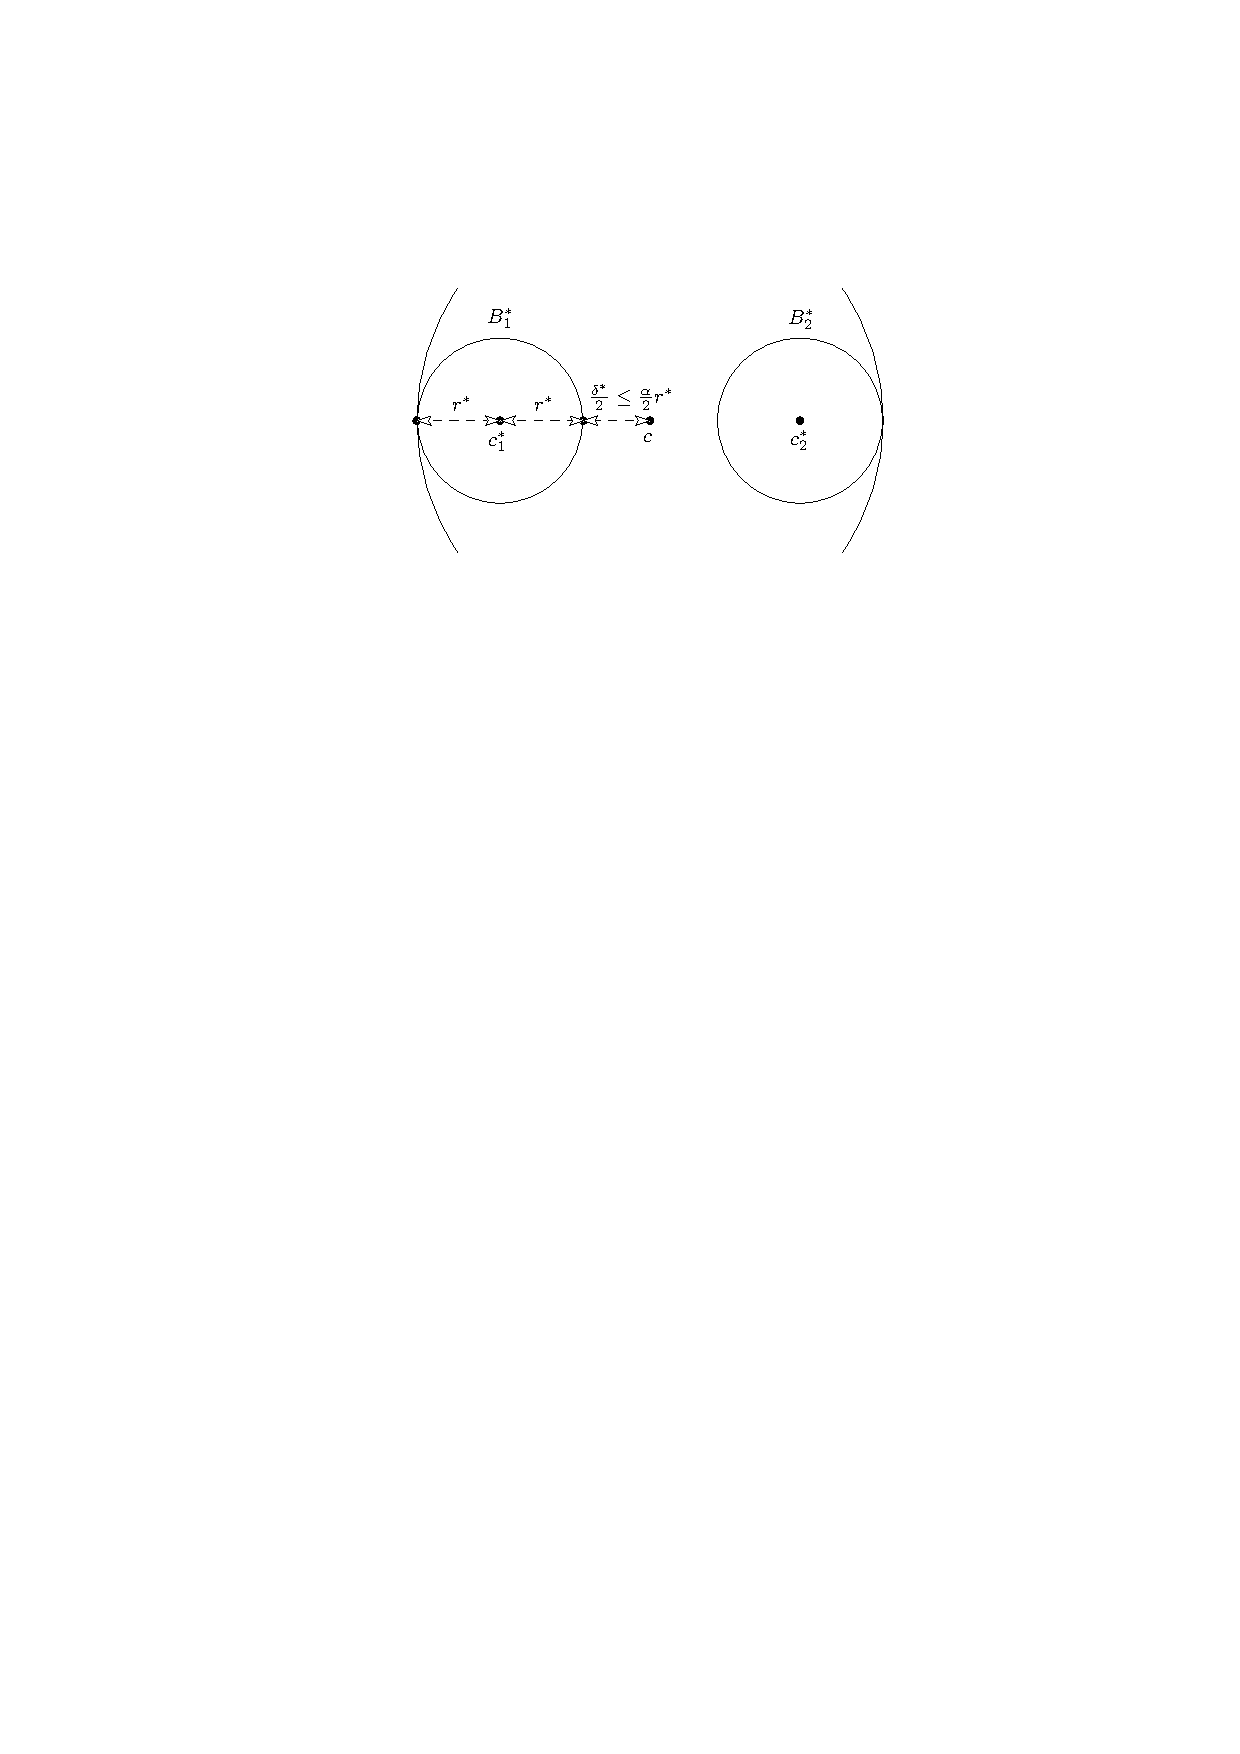
\includegraphics[width=19em]{figs/2lt1}
	\caption{Proof of Lemma~\ref{lem:2-approx}}
	\label{fig:2lt1}
\end{figure}

\noindent 
The following is a direct corollary of Lemma~\ref{lem:2-approx} and \Cref{thm:1-center}.

\begin{cor} \label{cor:4-approx}
	If $\delta^* \le \alpha r^*$, 
	\Cref{alg:1-center} computes a $(4 + \alpha)$-approximation to $r^*$. 
\end{cor}


%\begin{obs}
%\label{obs:2apr}
%Let $r_1$ and $k_0$ be two positive real numbers. Define $k=k_0 2^i$ to be the smallest real number satisfying the inequality $k \ge r_1$, where $i$ is a non-negative integer. Clearly, $k$ is a $2$-approximation for $r_1$.
%\end{obs}

%We maintains $m=\ceil{{1.2 (3 \alpha+12)}/{\eps}}$ candidate lengths.
%For each candidate length $r$, we run an instance of Algorithm~\ref{alg:smallc}. 

We use \Cref{alg:1-center} to find an estimate for $r$. 
Let $r_i$ be the radius calculated by \Cref{alg:1-center} after receiving
the $i$-th point, $p_i$.
Clearly, the sequence of $r_i$'s is increasing.
%We use a doubling strategy, similar o what is used in~\cite{zarrabi2008core}.
Let $k$ be an integer such that $2^{k-1} \le r_i \le 2^{k}$, and set $\ell_i = 2^{k}$.
%Let $l_1=r_1$ and $l_i=2^j l_1$, where $l_i$ is the smallest number satisfying $l_i \ge r_i$. 
Obviously, $\ell_i \le 2 r_i$,
and hence, by Corollary~\ref{cor:4-approx}, 
$\ell_i$ is a $(8 + 2\alpha)$-approximation to $r^*$.

We divide the interval $(0, 1.2 \ell_i]$ 
into $m=\ceil{{1.2 (3 \alpha+12)}/{\eps}}$ equal segments,
% (Figure~\ref{fig:findr}), then 
each of length $t_i = 1.2 \ell_i / m$.
Clearly,  $t_i \le (2\eps/3) r^*$.
Therefore, in the set
$R_i = \set{j \times t_i \provided j = 1, \dots, m}$,
there is at least one value $r$ for which the  
inequality $1.2 r^* \le r \le (1.2 + \frac{2\eps}{3})r^*$ holds.

%\begin{figure}[h]
%	\centering
%	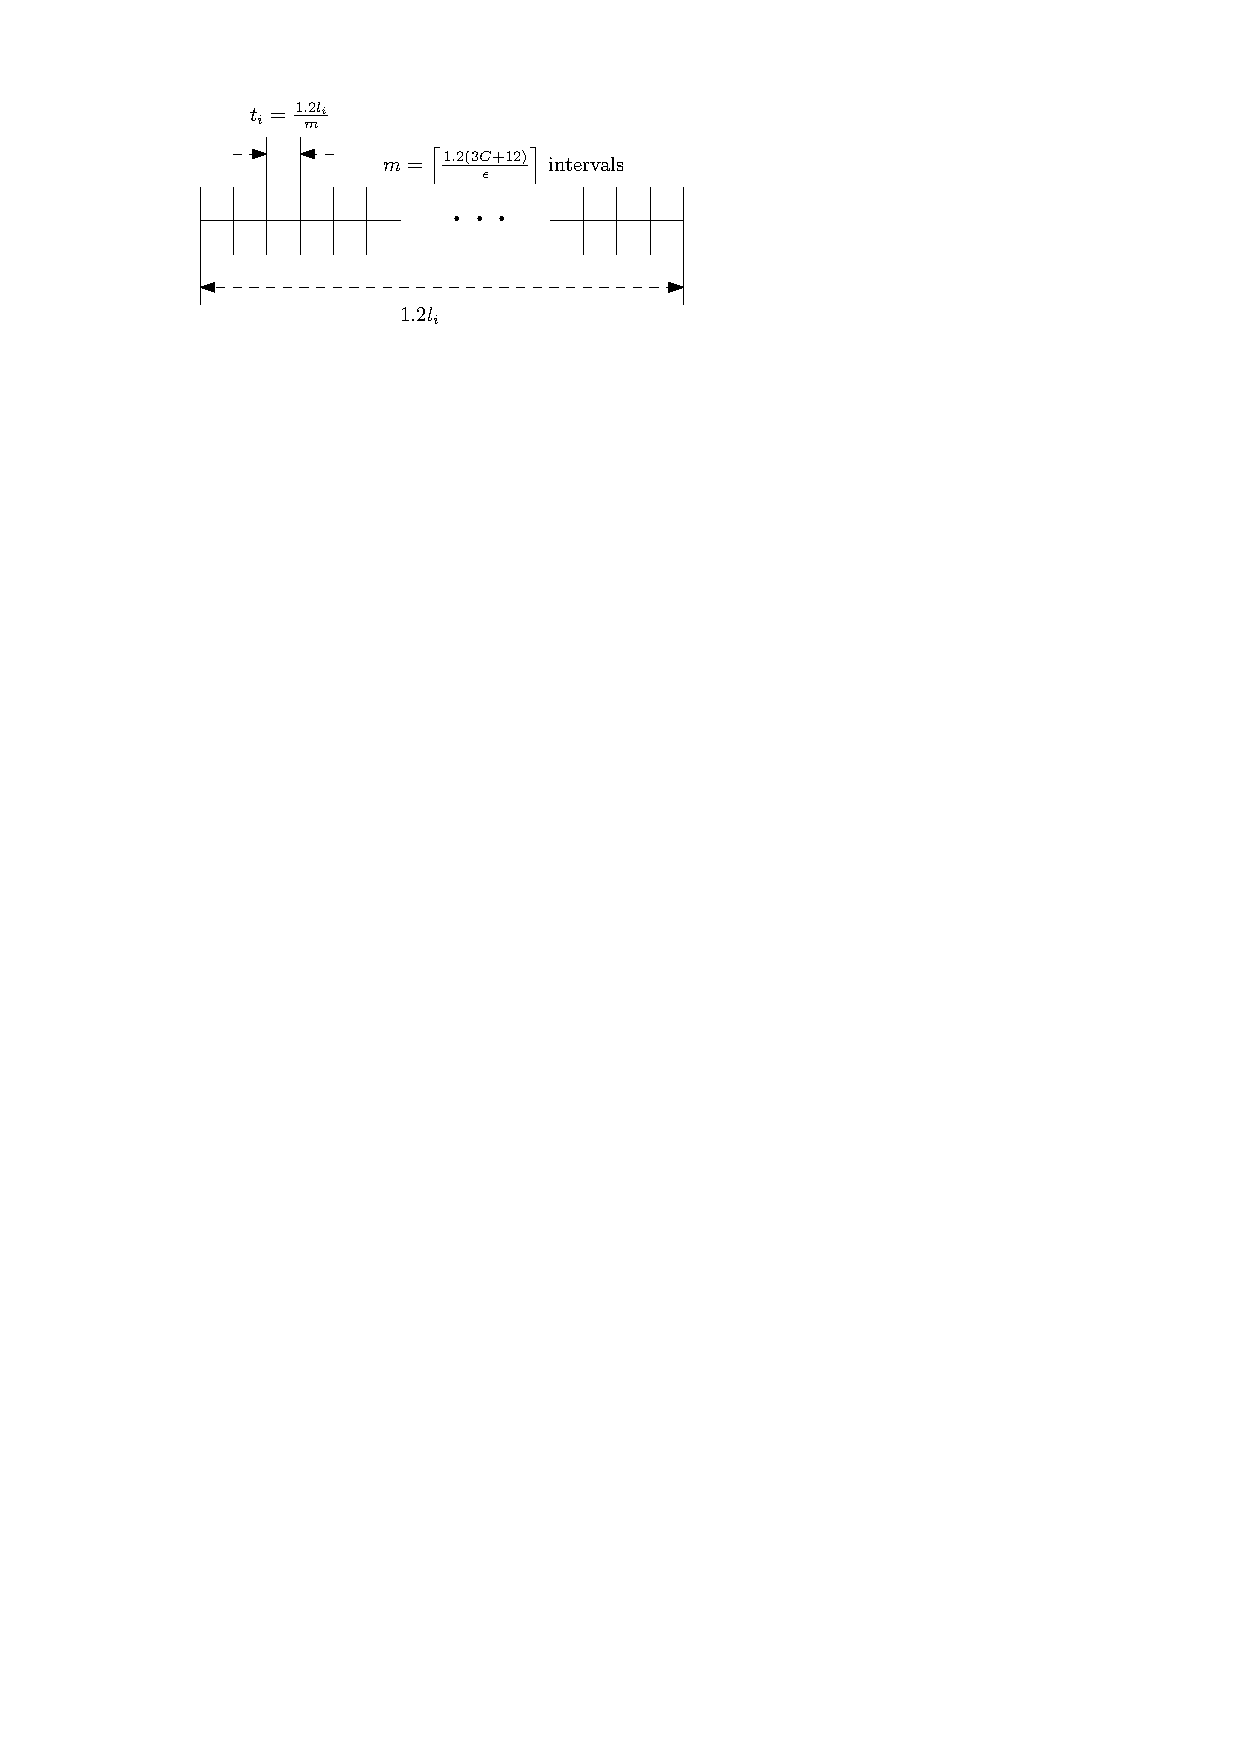
\includegraphics[width=21em]{figs/findr}
%	\caption{Subdivision of the interval $(0, 1.2 \ell_i]$}
%	\label{fig:findr}
%\end{figure}

%When the first non-zero radius is observed, $l_1$ is set. 
We run $m$ instances of Algorithm~\ref{alg:smallc} for each value $r \in R_i$ in parallel. 
%for all the previous points, which have been stored in a buffer. It is not hard to see that the space complexity for storing these points is $\O(z)$. 
Whenever a new point $p_i$ is added, 
if $\ell_i=\ell_{i-1}$, then $R_i = R_{i-1}$,
and the new point is inserted to all parallel instances. %corresponding to candidates in $L_i$. 
%Otherwise, Algorithm~\ref{alg:smallc} should be executed for all of the candidates in $L_i$, with all the points. But this is not achievable due to space limitations. 
If $\ell_i > \ell_{i-1}$, then the set $R_i$ has two types of values.
Those values in $R_i$ which are less than $1.2\ell_i$ are also present in $L_{i-1}$,
because $t_i / t_{i-1}$ is a positive power of 2.
For these values, we continue executing the corresponding instance.
If a value $r \in R_i$ is not present in $R_{i-1}$, 
then we have $r \ge 1.2 \ell_{i - 1} \ge \ell_{i-1}$.
%To overcome this problem, note that if the candidate $x_j=j \times t_i \in L_i$ is also in $L_{i-1}$, there is no need to start Algorithm~\ref{alg:smallc} over and the current execution will be continued. If $x_j \notin L_{i-1}$, then it is certain that $x_j \ge l_{i - 1}$ (Observe that $l_i=ul_{i-1}$, for some $u\in \mathbb{N}$). 
Since those points not lying in the candidate solution 
are saved in the buffer of Algorithm~\ref{alg:1-center} (which has size at most $z$), 
all non-outlier points of this algorithm lie in the candidate balls of Algorithm~\ref{alg:smallc} which has center $p_1$ and radius $l_{i-1}$. 
These outliers have been stored in a buffer. 
Since Algorithm~\ref{alg:smallc} maintains two balls with radius at least $r$, which one of them (say $B_1$) has center $p_1$, then all non-outlier points of Algorithm~\ref{alg:1-center} are in $B_1$ and so they do not make transition in Algorithm~\ref{alg:smallc} states.
Therefore, for a new value $r$, 
it suffices to execute Algorithm~\ref{alg:smallc} with only the outlier points in $B_1$,.
%Overall, we get the following result.

%\begin{theorem}
%\label{thm:1st-cmplx}
%Algorithm~\ref{alg:smallc} uses $\O(\frac{dz^3}{\eps})$ space, and takes $\O(\frac{dz^4}{\eps})$ and $\O(\frac{dz^3}{\eps})$ time for update and query, respectively.
%\end{theorem}


\end{document}
